\documentclass[class=article , crop=false, titlepage, twoside, multi={itemize, figure, verbatim}, float=false]{standalone}

\usepackage{import} % Required for importing other .tex docs.  (import uses everything bw Begin and End Doc)
\usepackage{float} % Required for specifying the exact location of a figure or table
\usepackage{graphicx} % Required for including images
\usepackage{wrapfig}
\usepackage[pdftex,breaklinks,colorlinks=true,linkcolor=black,citecolor=blue,urlcolor=red,linktocpage=false,pagebackref=true,filecolor=magenta]{hyperref}%http://www.tug.org/applications/hyperref/manual.html#x1-100003.6
\usepackage{cite}
\usepackage[toc,title,page]{appendix}
\usepackage{pdfpages} % enables loading a pdf into the doc
\usepackage{makeidx}
\usepackage{glossaries} % must be after hyperref
\usepackage{blindtext}
\usepackage{enumitem}
%\usepackage{caption}

%\setlist[description]{leftmargin=\parindent,labelindent=\parindent}

%\renewcommand*{\bibname}{References} % renames the bibliography

\newcommand{\HRule}{\rule{\linewidth}{0.5mm}} % Command to make the lines in the title page

\graphicspath{{img/}{GIS_ChampionSection/img/}{awardsChapter/GIS_ChampionSection/img/}{brandPart/awardsChapter/GIS_ChampionSection/img/}{img/}{pairedProgSection/img/}{methodChapter/pairedProgSection/img/}{methodPart/methodChapter/pairedProgSection/img/}{documentationSection/img/}{methodChapter/documentationSection/img/}{methodPart/methodChapter/documentationSection/img/}{docStorageOrgSection/img/}{methodChapter/docStorageOrgSection/img/}{methodPart/methodChapter/docStorageOrgSection/img/}{QGisSection/img/}{toolsChapter/QGisSection/img/}{servicePart/toolsChapter/QGisSection/img/}{ESRISection/img/}{toolChapter/ESRISection/img/}{servicePart/toolChapter/ESRISection/img/}{../../../../source/}{../../source/}{servicePart/applicationsChapter/treasurerSection/img/}}

%\setlength\parindent{0pt} % eliminates indents


\def\titlename{Versioning\\ \medskip\large Version Management in ArcGIS}

\title{\HRule % Horizontal Line added
\\[.4cm] % space
\begin{figure}[H] % included image
\begin{center}	% centered horizontally

\includegraphics[scale=.45]{GIS_Logo_better.jpg}
\end{center}
\end{figure}
\Huge \bfseries \titlename \\ % Title text
\HRule \\[.4cm] % Horizontal Line added
\author{\Large Allegan County GIS \\\Large www.allegancounty.org/gis} % defines author
}  % inputs common title
\setcounter{tocdepth}{5}  % subparagraph and down
\begin{document}% document begins


\ifstandalone
%\frontmatter % turns off chapter numbering and uses roman numerals for page numbers
\maketitle % creates title page and blank page after title page
\tableofcontents % creates TOC and blank page
\clearpage
%\mainmatter % turns on chapter numbering, resets page numbering and uses arabic numerals for page numbers
\fi

\subsection{Managing Geodatabase Versions}
\medskip 
\subsubsection[Version Queries]{\Large Version Queries}


\paragraph{SQL Queries \texorpdfstring{\\}{}}
Four queries of SDEversions, SDEstates, sdestatelineages, and SDEcompresslog

\begin{verbatim}

use AC_Pub
select name, owner, version_id, state_id, parent_name
, parent_owner from
 [AC_Pub].[dbo].[SDE_versions]
select * from [AC_Pub].[dbo].[SDE_states] order by state_id
select * from [AC_Pub].[dbo].[sde_state_lineages] order
 by lineage_name,
 lineage_id
select TOP(5) * from [AC_Pub].[dbo].[SDE_compress_log] order by
 compress_end DESC
 \end{verbatim}
Query of SDEversions and SDEstates
 
 \begin{verbatim}
 use AC_Pub
SELECT v.version_id,v.creation_time,v.creation_time,
 s.state_id, s.creation_time
FROM SDE_versions v
INNER JOIN SDE_states s ON v.state_id = s.state_id 

\end{verbatim}
\clearpage
\subsubsection[Orphaned Versions]{\Large Finding Orphaned Versions}
\paragraph{ID and delete orphaned geodatabase versions \texorpdfstring{\\}{}}
Follow the procedure:
\href{https://support.esri.com/en/technical-article/000010858}{Link to source}\\
Use SQL Server Management Studio to execute two queries and compare the results.
\subparagraph*{Step 1: \texorpdfstring{\\}{}}
Execute the query:
\begin{verbatim}
use AC_Pub
SELECT ObjectID, name from dbo.GDB_ITEMS where 
 TYPE='4ED4A58E-621F-4043-95ED-850FBA45FCBC';
\end{verbatim}
\subparagraph*{Step 2: \texorpdfstring{\\}{}}
Execute the query:
\begin{verbatim}
use AC_Pub
SELECT name from [dbo].[SDE_versions]
order by name

\end{verbatim}
Compare the tables
\paragraph*{}This graphic summarizes elements of the queries.
\begin{figure}[h!]
\centering
    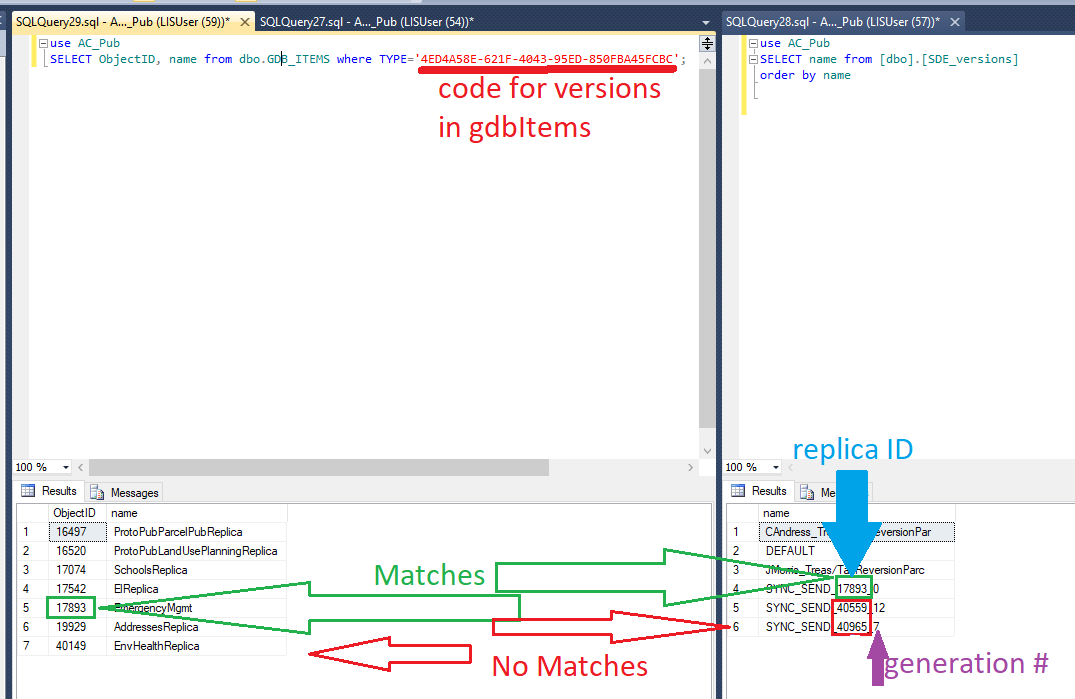
\includegraphics[width=.95\textwidth]{findOrphanReplicaSystemVersions.png}
\caption{Find Orphan Versions}
\end{figure}
Note the items from step two that have no match in step one.
\clearpage

\paragraph*{}Orphaned versions can be removed by name in ArcGIS
\begin{figure}[h!]
\centering
    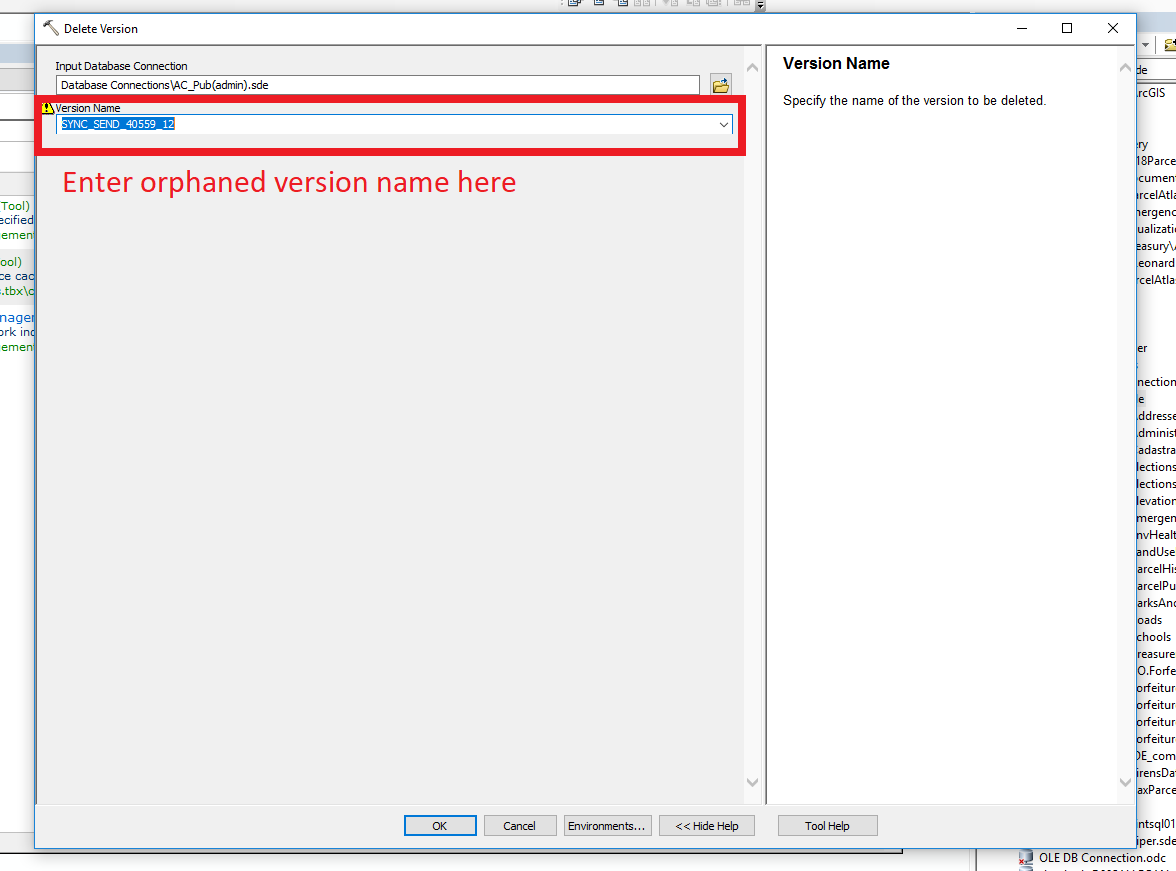
\includegraphics[width=.95\textwidth]{deleteOrphanVersion.png}
\caption{Delete Orphan Versions}
\end{figure}
\clearpage

\end{document}